\clearpage
\section{Project Background}
\subsection{Business Problem and Opportunity}
SITA is probably one of the most strategic of Government agencies, not only is it positioned to allow Government departments to provide services efficiently and cost effectively, it ensures that there is co-ordination across Government. One of the core functions is to build and deploy e-government services. This includes not only the development, but also the management and support  of all e-government services. In a way SITA can be seen as the largest IT company in the country, possibly the continent, as Government is the largest user of IT systems, with the largest client base in the country. SITA is largely seen as an external service provider, with many Government departments having their own internal IT divisions. This in itself introduces a number of challenges, including conflict between departmental IT teams and those working on projects through SITA. Many departmental heads would also view SITA as merely a cost centre to be used within their own departments. 
%\client has selected specific departments where analysis work and requirements were conducted in order to deliver an e-government solution for the department and government as a whole.
One of the key contributions that \client would undertake is to deliver e-government services. 
The challenge lies in the manner in which such solutions would be implemented in-order to maximize reuse; automate as far as possible; and allow for greater levels of management by non-technical staff.The approach that would be undertaken in order to achieve such goals would follow a model-driven approach;  and would  ensure that the overall solution meets the demands of all stake-holders; in a transparent manner.

%The solution would thus be to build a Enterprise Architectural type for e-government.
%This would be composed of a number of layers; the first being the Architecture Model
%that would support the e-government strategy for a given department; a suitable
%Model Driven Architecture to support the design and implementation of e-government
%services; and lastly a Technological Model to provision the infrastructure to support the
%e-government services. 
%\clients\: mandate is to build and deploy e-government services. \client has to support and manage the IT needs of all government departments. Thus in a very general view \client can be viewed as an external IT department for all of government. This type of relationship even in the private sector introduces a number of challenges; firstly any given department would view \client as a cost center in it's own structure. For many departments IT is the largest stake of their budget, and would further feel that \client has more power than their own internal structures. Furthermore for a non-technical person to understand the value of \client can be quite daunting and frustrating. Thus the idea would be to build a \textit{Enterprise Architectural Style} for e-government.
%This would be composed of a number of layers; the first being the \textit{Architecture Model} that would support the e-government strategy for a given department; a suitable \textit{Model Driven Architecture} to support the design and implementation of e-government services; and lastly a \textit{Technological Model} to provision the infrastructure to support the e-government services. Finally we would propose \textit{Platform Specific Models} for each of the layers to manage and implement the e-government services.
%\clearpage
%\slist
%\spit Build an Enterprise Architecture Style for e-government
%\slist
%\spit For a given department build an \textit{Architecture} Model that would deliver on the given departments e-government strategy.
%\spit Establish the current status of the department by accessing the resource capacity and the state of technology.
%\spit Define the method to migrate the department from it's current state to the targeted Architecture Model
%\elist
%\spit Development Model: Model Driven Approach 
%\slist
%\spit Automate the design of the human interaction component of the e-government strategy.
%\spit Automate the design and implementation of the master data for the given department.
%\spit Automate the deployment and management of the e-government components for the given department.
%\spit Provide a validation engine and supporting infrastructure to allow the Department itself to maintain and manage their e-government components.
%\elist
%\spit Provide a technology stack that would support e-government
%\slist
%\spit Technology drivers Government's Objectives; Data Management; Technology Best of Breed
%\elist
%\elist
%Currently \client has an OpenJIG, which provides a technology stack to deploy applications supported by UI, Business Logic and persistent store. 
%However the reality is that there exists a number of e-government services across the various departments, in order to maintain a consistent look and feel as well as minimize the resource requirements we would like to automate this process as far as possible. Furthermore such automation would also ease the burden of maintenance. Since some services would cross department lines, collaboration and integration techniques would need to be employed in order to maintain data governance and ensure quality of service. Another important facet of e-government services is that they always maintain compliance to legislation and policy; thus we further propose to build a validation engine based on domain knowledge.
\subsection{Project Recommendation}
The project will be developed as a hybrid of a research project and an implementation project. As the name suggests the research component would deliver on the modeling and theoretical principles to support the solution. The applied component would provide the implementation infrastructure to deliver on the solution. In order to be as efficient as possible; some of these activities may be executed in parallel.
\\
\\
In Figure \ref{AV} we present a high-level view of the environment, note that this project is concerned with the area marked in red. The assumption is that the developers would produce the relevant artifacts to be deployed onto the Java Platform. The Java Platform is broken up into the various layers, each layer is composed of the generic components/models and it's companion is the technology specific layer.
The artifacts in some respects maybe translated into appropriate components for the target platform, or in some scenarios modifications to the toolchain would be required to efficiently deliver e-government services.
\begin{figure}[h!]
  \caption{Technical Architecture View of Java Platform}
  \label{AV}
  \centering
    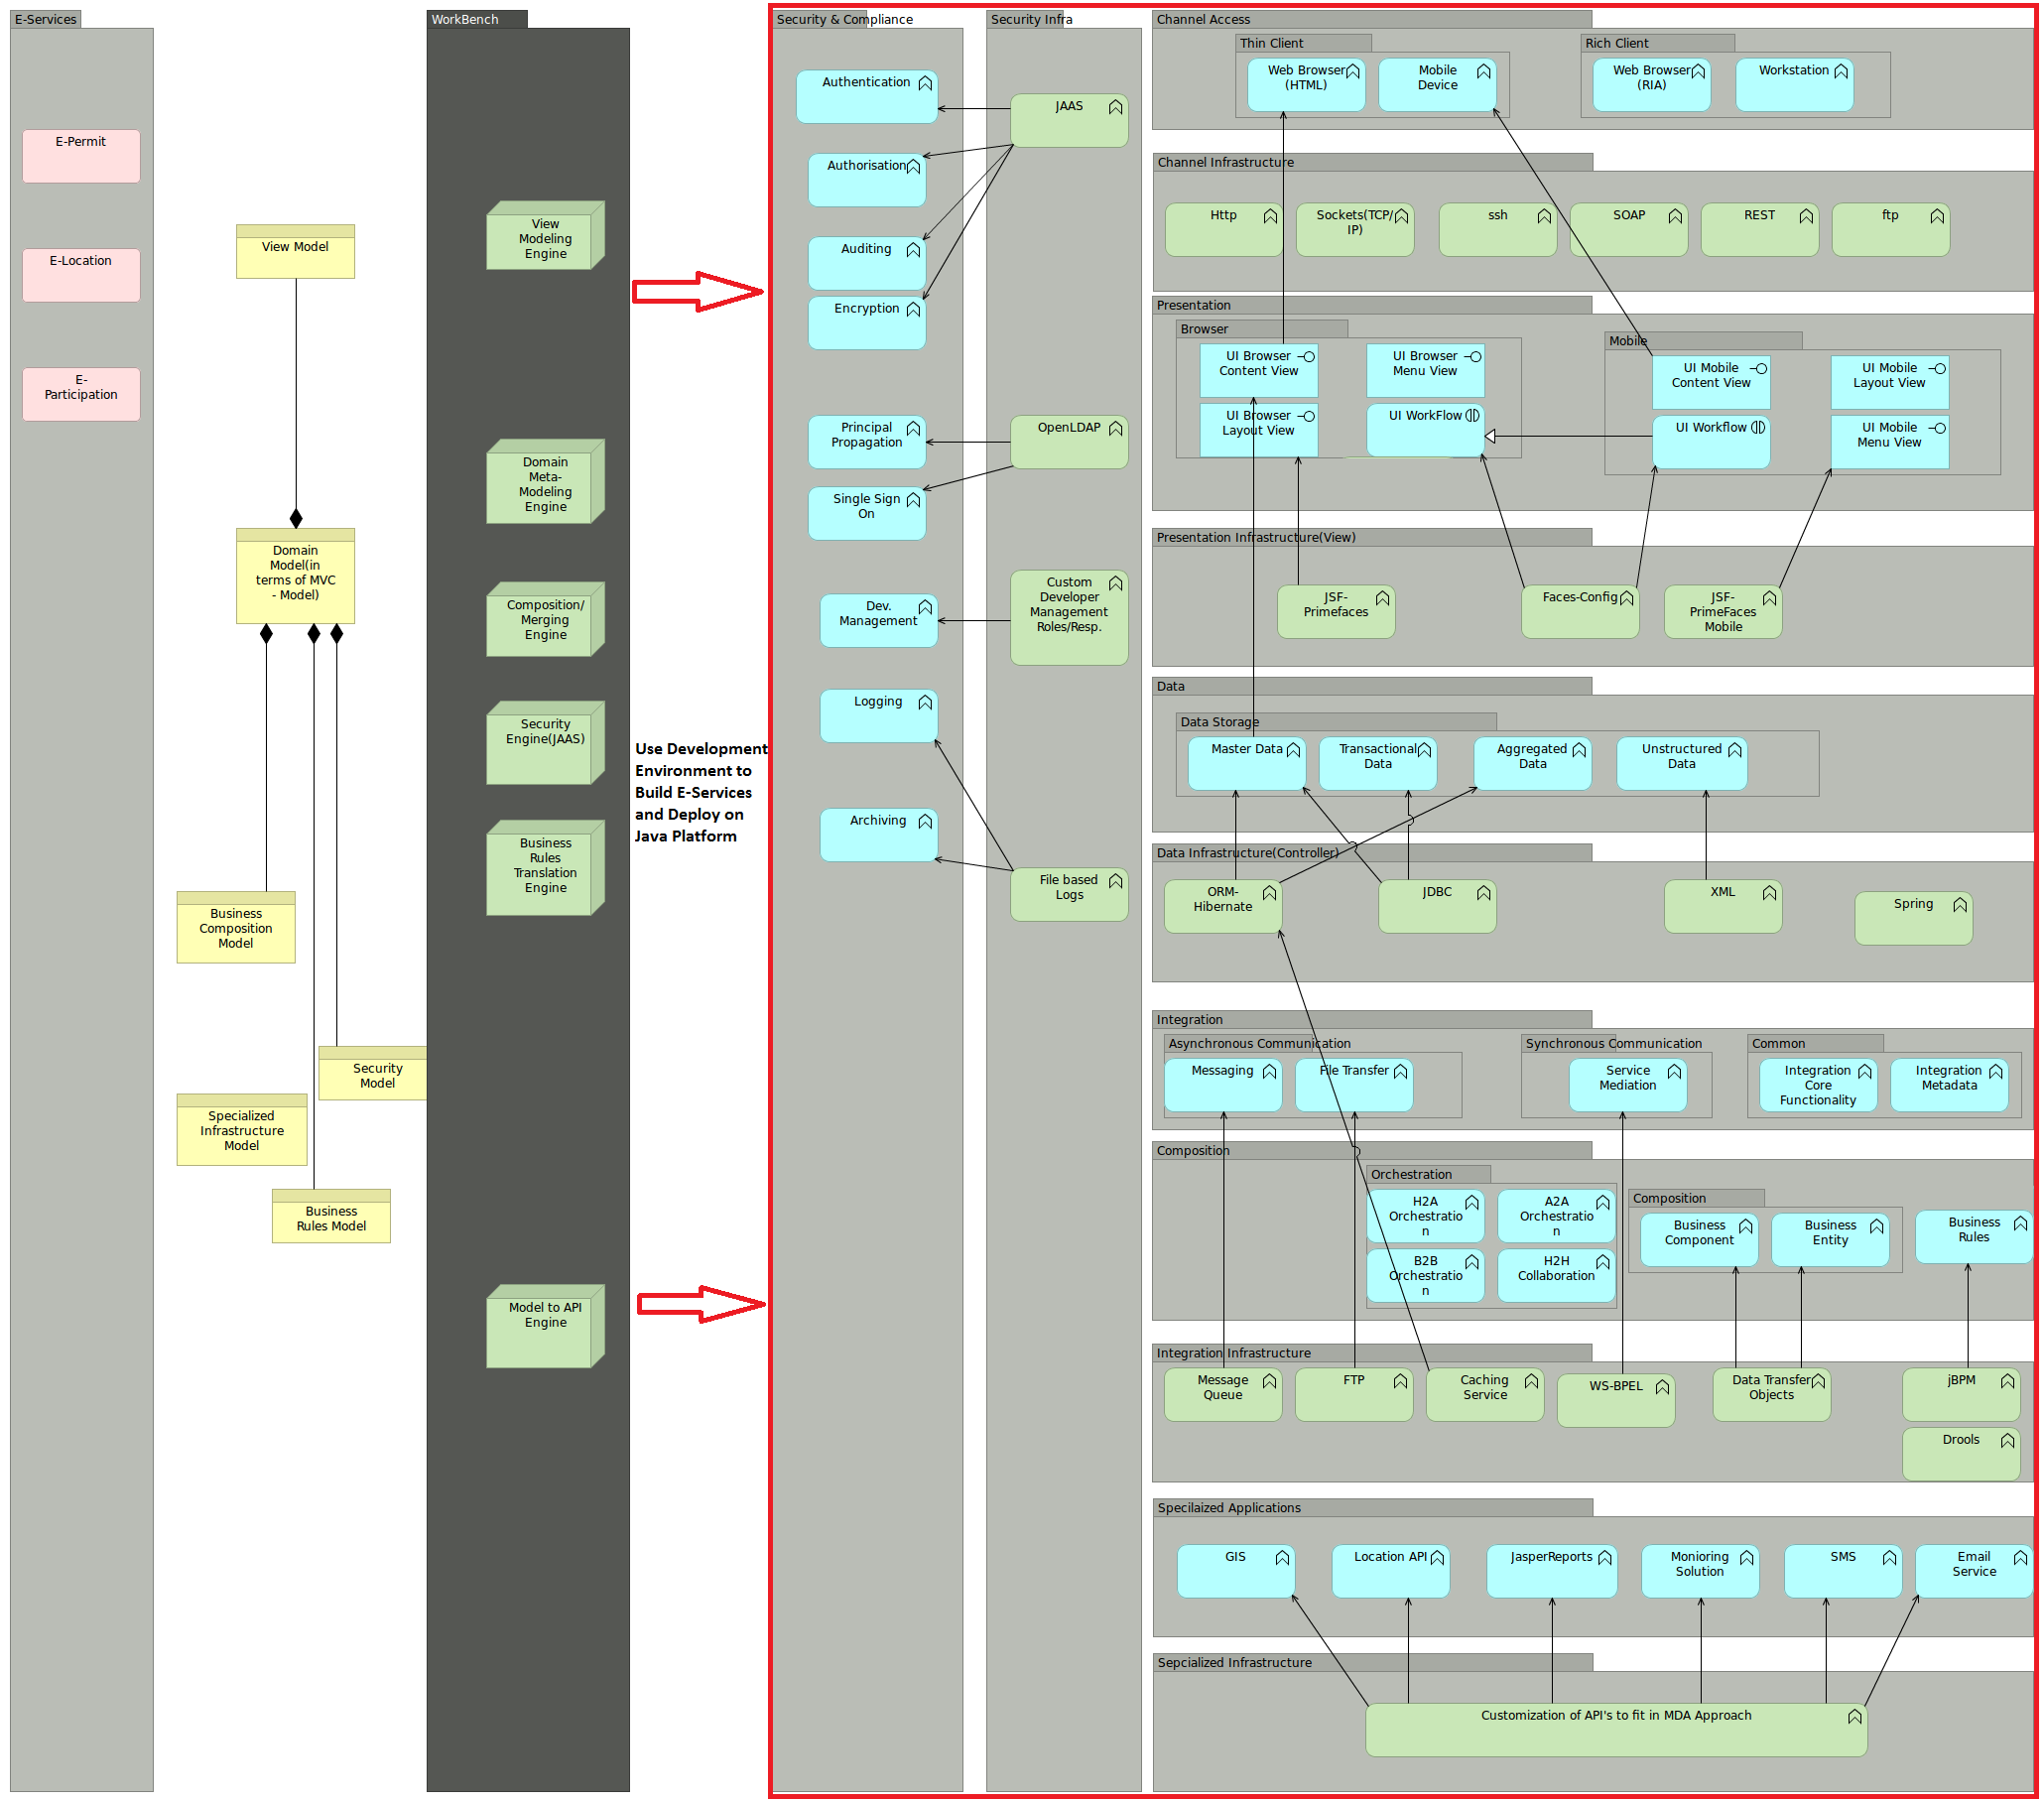
\includegraphics[width=0.9\textwidth]{images/javaplatform1.png}
\end{figure}
\clearpage


The initial phase would be:
\slist
\spit Planning and Analysis Phase
\slist
\spit An initial assessment would need to be conducted in order to establish the suitability of the requirements information
\spit A translation map would be designed and implemented in order to migrate the requirements definitions into model structures
\spit An analysis would be conducted in order to understand the types of modeling techniques to be employed 
\spit An analysis would be conducted in order to validate the current toolchain to deliver on the solution
\spit Project Planning and Initiation phase
\elist
\spit Build the "Development Infrastructure" for the E-government Services
\slist
\spit Build a repository to store "Model Types" that would support the department's e-government services.
\spit Enhance the toolchain to support "Model Types" to support composition and merging at the different layers in the Technology stack
\elist
\spit Build and implement the "Technology Infrastructure" to support e-government services 
\elist
\subsection{Resource Contingent}
\vendor proposes to make available the following skill types to execute the project:
\slist
\spit Enterprise Architect
\spit Project management.
\spit Requirements Engineer
\spit Technical Architect
\spit Solution analysis 
\spit Solution design
\spit Solution development
\spit IT Governance
\spit Solution testing
\elist
\subsection{Standards and Procedures}
The following standards and/or procedures have and will be consulted:
\slist
\spit TOGAF- Open Works Group
\spit GWEA - Government Wide Enterprise Architecture
\spit \gls{EMF} and associated Eclipse Standards supported by the eclipse community, thereby immediately benefiting from a large toolchain set.
\spit Common Variability Language, An OMG Standard
\elist
